\documentclass[onesided,a4paper,10pt]{article}


%\usepackage[]{}
%\usepackage[]{}
\usepackage[english]{babel} %english, 
\usepackage[utf8x]{inputenc} %latin1, utf8x, utf8

\setcounter{secnumdepth}{3}
\setcounter{tocdepth}{3}

\renewcommand*{\familydefault}{\rmdefault}

\usepackage{longtable}
\usepackage{graphicx}
\usepackage[hidelinks]{hyperref}
\usepackage{url}
\usepackage{lastpage}
\usepackage{multicol}
\usepackage{fancyhdr}
\pagestyle{fancy}
%\renewcommand{\chaptermark}[1]{\markboth{#1}{}}
%\renewcommand{\chaptermark}[1]{\markright{\thesection\ #1}{}}
%Even pages
\fancyhead[LE]{\leftmark}
\fancyhead[CE]{}
\fancyhead[RE]{}
\fancyfoot[LE]{\thepage\ of \pageref{LastPage}}
\fancyfoot[CE]{}
\fancyfoot[RE]{}
%Odd pages
\fancyhead[LO]{\thesection}
\fancyhead[CO]{}
\fancyhead[RO]{\emph{\thechapter}}
\fancyfoot[LO]{}
\fancyfoot[CO]{}
\fancyfoot[RO]{\thepage\ of \pageref{LastPage}}

\usepackage{color}
  %\definecolor{}{rgb}{0.0, 0.0, 0.0}
  \definecolor{xGreen}{rgb}{0.0,  0.6, 0.0}
  \definecolor{xGray} {rgb}{0.5,  0.5, 0.5}
  \definecolor{xMauve}{rgb}{0.58, 0.0, 0.82}

\usepackage{listings}
\lstset{
  language          = [ISO]C++,%Java, Matlab, XML HTML, Python, PHP, Ruby, Perl,
                               % bash, [x86masm]Assembler, [ANSI]C, [Sharp]C, 
                               %[Visual]C++, [GNU]C++, Basic, 
  breakatwhitespace = false,
  breaklines        = true,  
  backgroundcolor   = \color{white},
  basicstyle        = \footnotesize,
  captionpos        = b,  
  commentstyle      = \color{xGreen}, 
  keywordstyle      = \color{blue}, 
  numberstyle       = \tiny\color{xGray},
  stringstyle       = \color{xMauve}, 
  deletekeywords    = {...},
  escapeinside      = {\%*}{*)}, 
  extendedchars     = true,  
  frame             = none,
  keepspaces        = true,  
  morekeywords      = {*,...},
  numbers           = left,  % where (none, left, right)
  numbersep         = 5pt, 
  rulecolor         = \color{black},
  showspaces        = false, 
  showstringspaces  = false, 
  showtabs          = false,
  stepnumber        = 2,  
  tabsize           = 2, 
  title             = \lstname
}


\title{ {\Huge Assignement 1 \\\Large Group 8}}
\author{ \Large Miranda, Adrian and Magnus }
\date{ \Large Report generated: \textbf{\today }}

\begin{document}
	\maketitle
	\tableofcontents
	\clearpage
	
\section{Task A}
For our environment we decided to make a graph structure based upon a set of
"Cells", which has links to its four adjacent neighbors, left, right, up and 
down. By doing so we can make intricate shapes and save memory in doing so. By
using a graph structure we can create complex environments, regardless of size,
with different shapes and connect multiple environments with passageways and
different elements within the environment.

By doing so we also ensure that the agent can easily move from and to cells by
simply going to an adjacent cell, using the links.  Since it is a graph
environment it is also possible to implement graph searching algorithms to find
solutions to different problems.

The environment is very modular because it consists of seperate "cells" which
links to one another.  As shown in figure \ref{fig:env}

\begin{figure}[h] \label{fig:env}	\centering
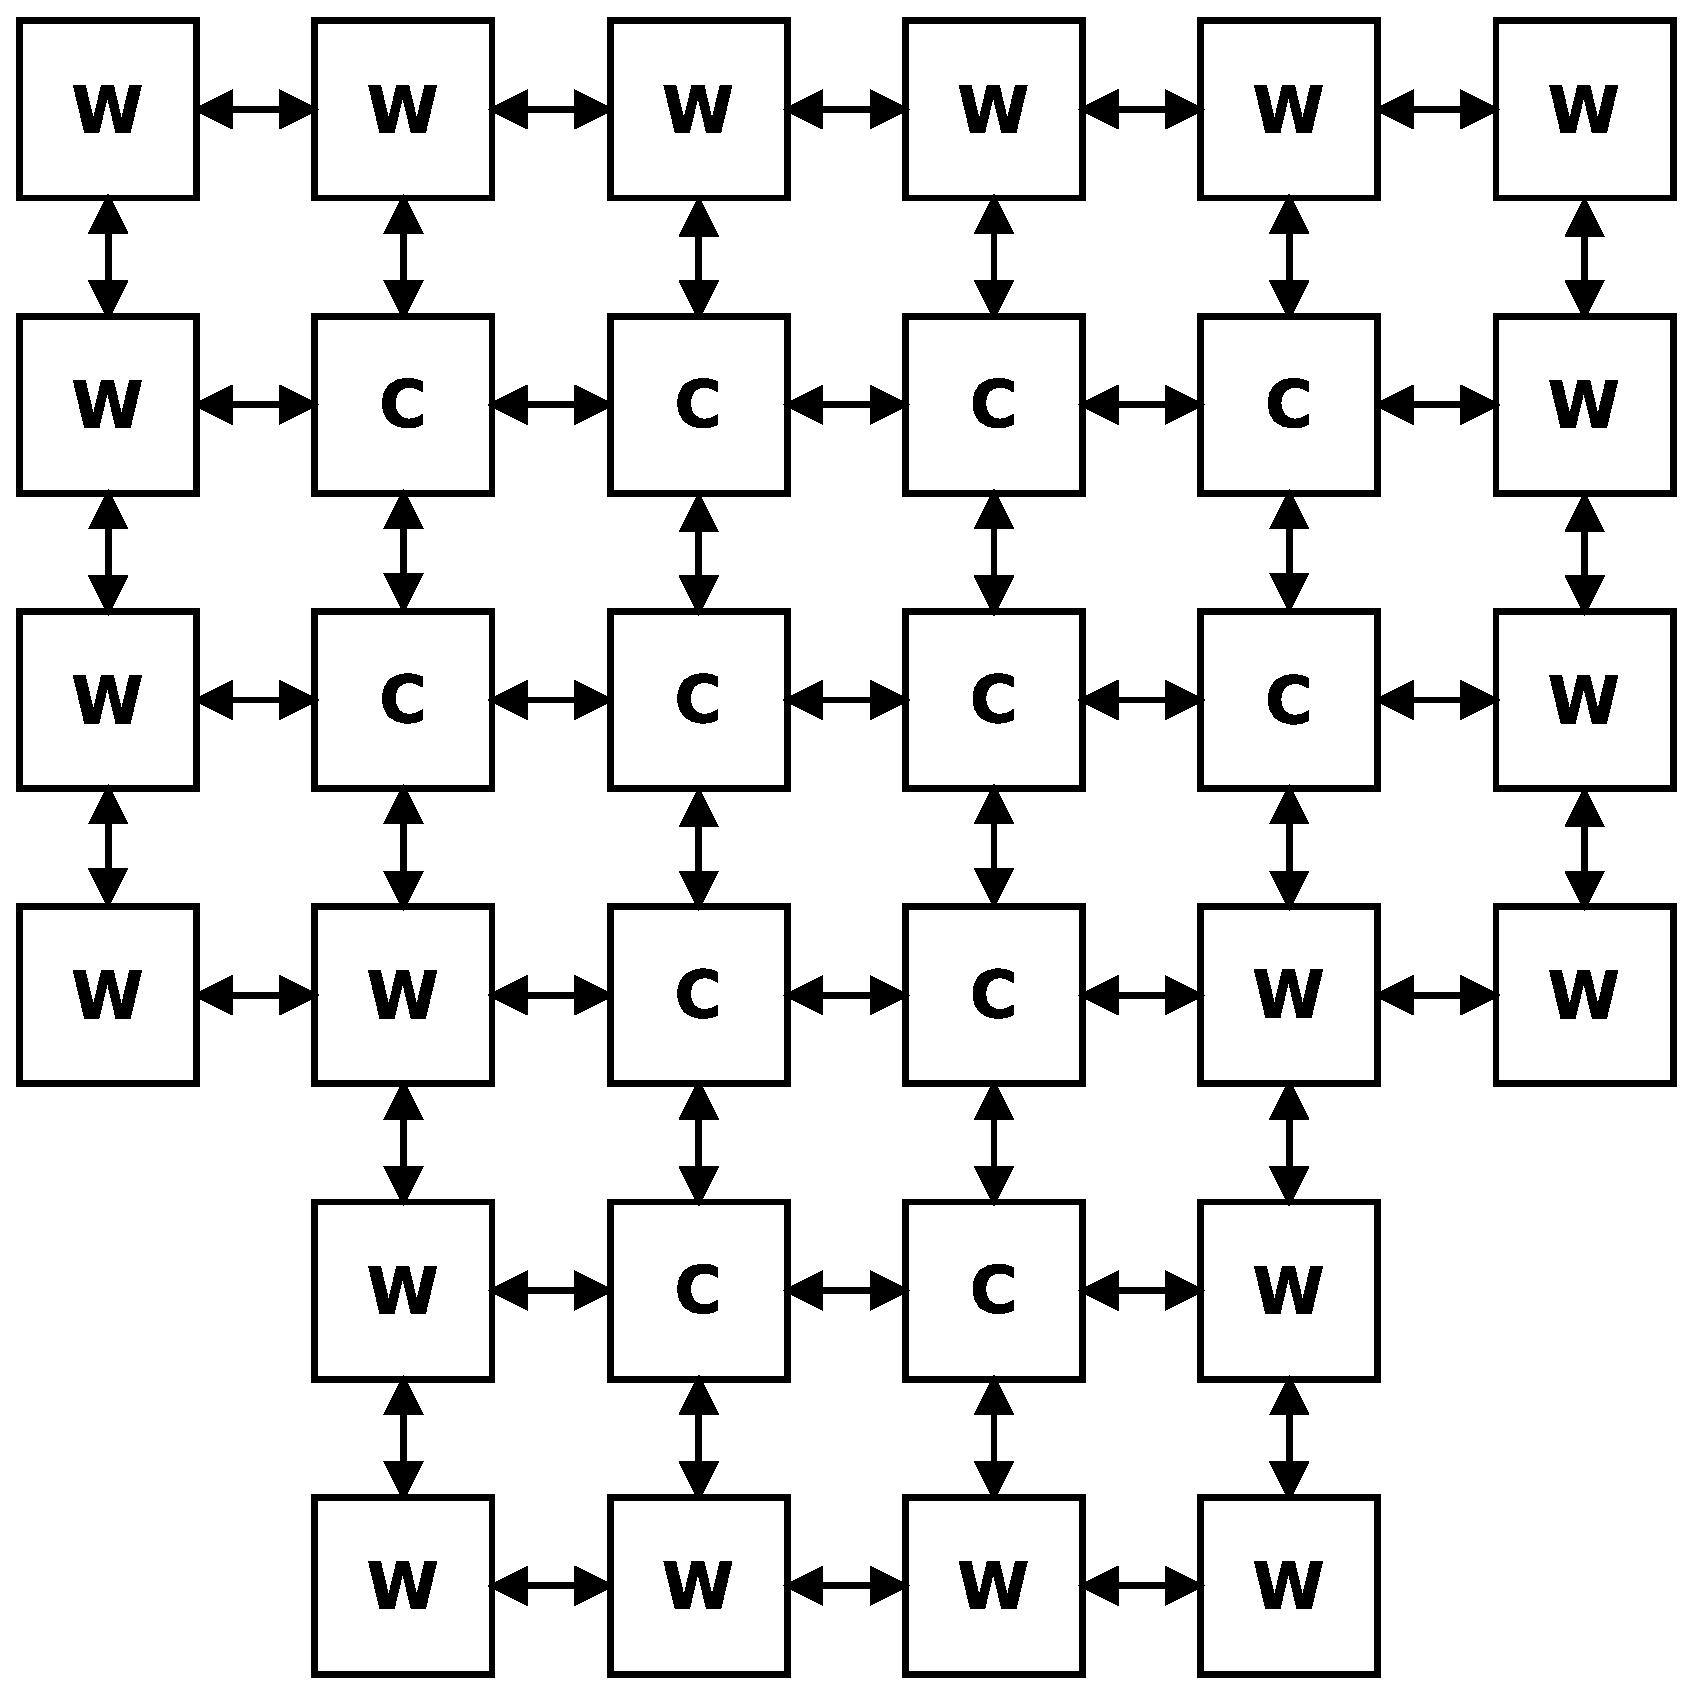
\includegraphics[width=0.6\textwidth]{environment}
\caption{Depiction of an environment}
\end{figure}

\subsection{Cell}
A cell is shown in figure \ref{fig:cell}. A cell is an object that holds
certain information about its current state and links to each of its four
adjacent cells.  The information it holds are:
\begin{description}
\item[key:] 
This integer holds the unique ID of the cell, which is used to search identify 
it during searches. It is specially used during creation of the environment, 
using the createMap() function in "main.cpp";

\item[type:]
Depicts the type of cell by using an integer.  The global ENUM variable sets the
different types as OPEN, WALL and OBSTACLE which is later used in comparisons.

\item[dirty:]
This boolean value states whether or not the current Cell is dirty or not. If it
is true the agent should suck it.

\item[age:]
This holds the information of how many steps it's been since it was last
cleaned.

\item[visited:]
Holds the state of wether the Cell has been visited by the agent. It is not
currently used, but would be to great help in a potential algorithm. For
instance if you need to mark visited cells to avoid getting stuck in a loop .

\item[neighbor:]
This is the four links to the adjacent neighbors; left, right, up and down. The
neighbors can either be set or be NULL if they are the border cell.

The setNeighbors function will set all four neighbors by calling the
setNeighbor(int, Cell*, Cell*) which sets the Cells neighbor as indicated by the
integer(LEFT, RIGHT, DOWN or UP).  Then this function will in return call the
new neighbors setNeighbor(int, Cell*) which creates a link back to the current
Cell.
\end{description}

\begin{figure}[h] \label{fig:cell}	\centering
\includegraphics[width=0.5\textwidth]{cell}
\caption{Depiction of a cell and its information}
\end{figure}


\subsection{Environment}

As statet the environment is built up by creating and linking Cells together in
a graph structure. The environment is created by the createMap() function which
reads the graph structure from a file.  The file format is a set of Cells
described by their type and left and right neighbor in a specific order starting
from the far left side.

The file format is [TYPE] [LEFT] [RIGHT]. Where the type is either W for wall, C
for open space and O for an object. LEFT and RIGHT is an integer value
describing the key of the Cell to link to.  This is critical that the keys are
correct and allready created.  The keys are automatically generated during
creation, starting at 1.  Because of this it is important that the cells are
created in correct order so the key exists when linking a new Cell.  If the
RIGHT/LEFT is 0 it will set the neighbor to NULL.

\subsection{Creation}
The Cells are contained in the form of two representations.  The first is the
graph where cells link to each other, and the second is a list which has a
pointer to a Cell and a pointer to the next member of the list, see figure
\ref{fig:list}. The purpose of the list is to enhance the searching speed when 
finding an existing Cell.

Creation of the environment is done by reading the file with the mappings and
creating the new cell without any neighbors. Then it sets the neighbors. After
this it will create the new list-member with a pointer to the Cell-object.

Then this list member will be added to the list before continuing creating the
rest of the cells.

To get a hold of the environment and the list there are created to static
variablels which holds the first element of the list and the first Cell.

\begin{figure}[h] \label{fig:list}	\centering
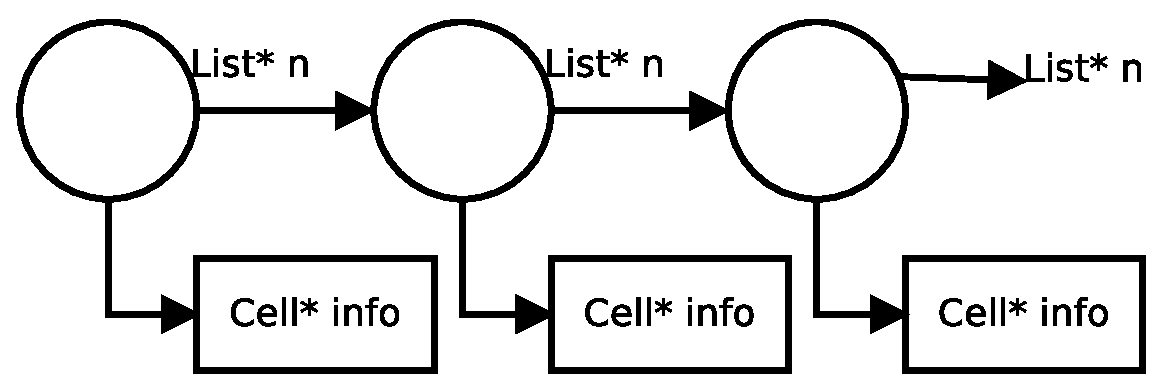
\includegraphics[width=0.75\textwidth]{list}
\caption{Depiction of the list representation of cells}
\end{figure}


	
\section{Task B}
The agent is an object with a finite set of rules that will move around the
environment.  Our simple reflex agent requires the assumption that the
environment is a rectangular shape, surrounded by walls and free of obstacles.

We've also contemplated an algorithm that will recursively move around the
environment and mark the visited cells to avoid an endless loop situation.

The problem with the recursive algorithm is that the agent has to manage the
counters and initiate the performance calculation itself.

\subsection{Agent}
The agent has the following attributes, some are not used during the algorithms
but will be needed for other types of algorithmic designs. See figure
\ref{fig:agent_uml} for the uml description of bot attributes and functions.

\begin{figure}[h] \label{fig:agent_uml}	\centering
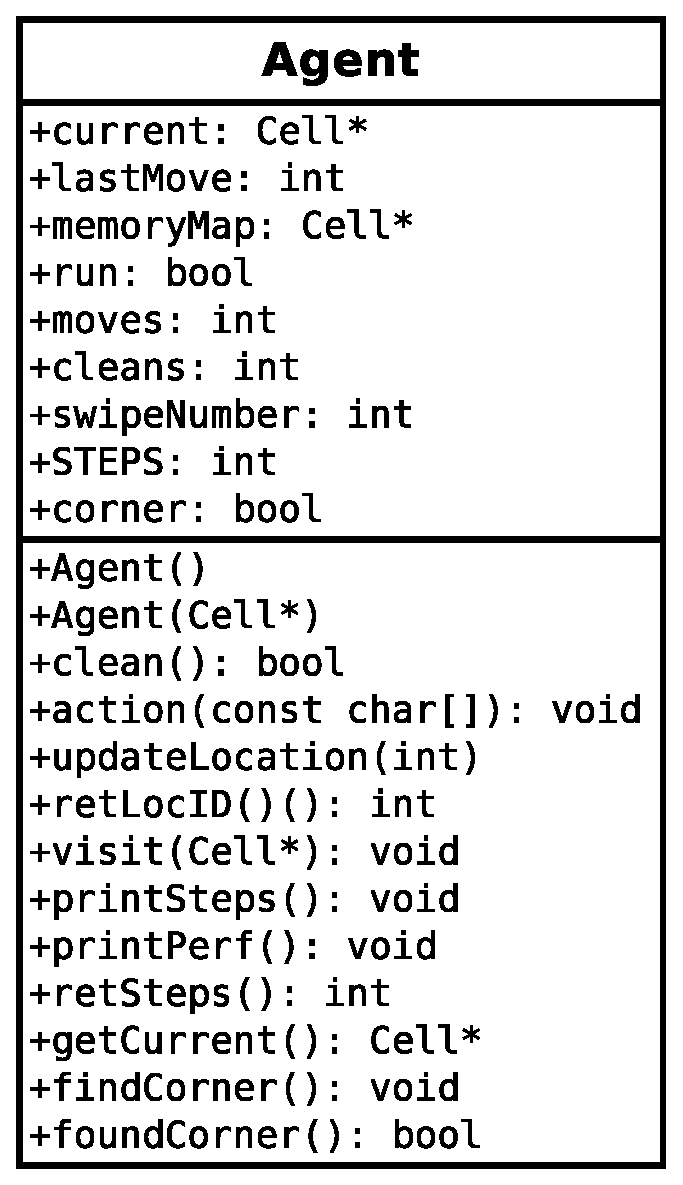
\includegraphics[width=0.35\textwidth]{agent_um}
\caption{UML description of an Agent object}
\end{figure}

\begin{description}
\item[current:]
	This is a Cell* pointer which will point to the current location of the agent.
	Whenever the agent moves the "current" attribute has to be changed to point to
	the new Cell object, which is done by calling the current locations getNeighbor
	function which returns the Cell* pointer to its neighbor.
\item[lasMove:]
	This is an integer describing the direction of the last move made. The moves
	possible are described as a global ENUM as "LEFT", "RIGHT", "UP" and "DOWN".
	By utilizing this the agent can avoid going back to its previous location,
	unless nessecary
\item[memoryMap:]
	This is not currently in use, but can be used to start building a map of the
	environment inside the robots head.  This is set as a Cell, but should be made
	into a different object type with minimal information.
\item[run:]
	This is a boolean value which could  be used to make the agent power down and
	stop cleaning/moving.  Which could be usefull if the room will never get dirtu
	again, since it could stop when finding the second corner.
\item[moves:]
	This is a counter which counts how many movements the agent has performed
	during its run.  This is used when displaying the performance rate of the
	agent.
\item[cleans:]
	This is a counter of how many cells the agent has cleaned during its run. The
	attribute is used during display of the performance rate.
\item[swipeNumber:]
	This is an integer that describes which way the agent is supposed to move.
	The agent will increment this counter each time it hits a wall and thereby
	switch moving to a side. 
\item[STEPS:]
	This is an internal counter to count the number of times the agent has
	perfomed an operation and is used to stop the agent after a certain amount of
	operations.  The counter is for creating an equal amount of movements during
	performance testing.
\item[corner:]
	This is an boolean value describing whether or not the corner has been found.
	The value is set to false during initation and true when the corner is found.
	By utilizing this we can switch from performing the find  corner algorithm to
	our movement algorithm.
\item[perf:]
	Integer holding the current performance value of the agent.
\end{description}

\subsection{Two cell environment}
This is the base test for running our agent in an environment.  The environment
is two cells, cell A and B. These cells links to each other and the main running
function controls the agents movements in the following manner. If the agent is
still running, it will start checking if the current cell is clean and clean it
if nessecary.  If it is clean it will check if the left neighbor exists and move
there if it does.  If the left neighbor is non-existant it has hit the end and
should start going to the opposite side. Thus we change the way to move and it
starts moving to the right. When it hits the end of the right cell it will stop
the agent from running or pause it untill it is restarted or the current
location becomes dirty.

To optimize the test case one could check each neighbor of the current location
to see wether it is at the left or right end and then possibly improve the
performance.

Performance is counted by awarding one point for each clean cell at the end of
each step.  It is also seen in context to the amount of movements and the amount
of times the agent cleans a location.

\subsubsection{Performance test - initial dirt}
This performance test was to test the very simple algorithm for two neighboring
cells, which did not become dirty after being cleaned.  We ran each test two
times for each type of initial state. The states was [clean, clean],
[clean,dirty], [dirty,clean], [dirty,dirty].  For each of these states we ran
the test starting in cell A and cell B.

\begin{longtable}{p{0.05\textwidth} p{0.075\textwidth} p{0.075\textwidth} 
									p{0.05\textwidth} p{0.075\textwidth} p{0.075\textwidth} 
									p{0.13\textwidth}}
Start	& A & B & Steps & Moves & Cleans & Performance \\\hline
A & Clean & Clean & 1000 & 1 & 0 & 2000 \\
B & Clean & Clean & 1000 & 2 & 0 & 2000 \\
A & Dirty & Clean & 1000 & 1 & 1 & 2000 \\
B & Dirty & Clean & 1000 & 2 & 1 & 1999 \\
A & Clean & Dirty & 1000 & 1 & 1 & 1999 \\
B & Clean & Dirty & 1000 & 2 & 1 & 2000 \\
A & Dirty & Dirty & 1000 & 1 & 2 & 1998 \\
B & Dirty & Dirty & 1000 & 2 & 2 & 1998 \\
\end{longtable}



\subsection{Simple algorithm}
	This algorithm is good for simple environment shapes, squares or rectangles without many obstacles inside.
	
	The algorithm starts by placing the agent in the bottom left corner, as shown on the picture. 
	By doing this we are certain of the position of the agent and it can move more conciusly.
	This part of the algorithm is pretty simple, the agent when created will only move towards the bottom.
	Once it hits the wall and retreats it will only go to the left.
	Again, when the left wall is hitted the agent knows its exact location.
	This part of the algorithm is only done the first time it executes.
	Once it finds the bottom left corner once its enough.

\begin{figure}[h] \label{fig:corner}	\centering
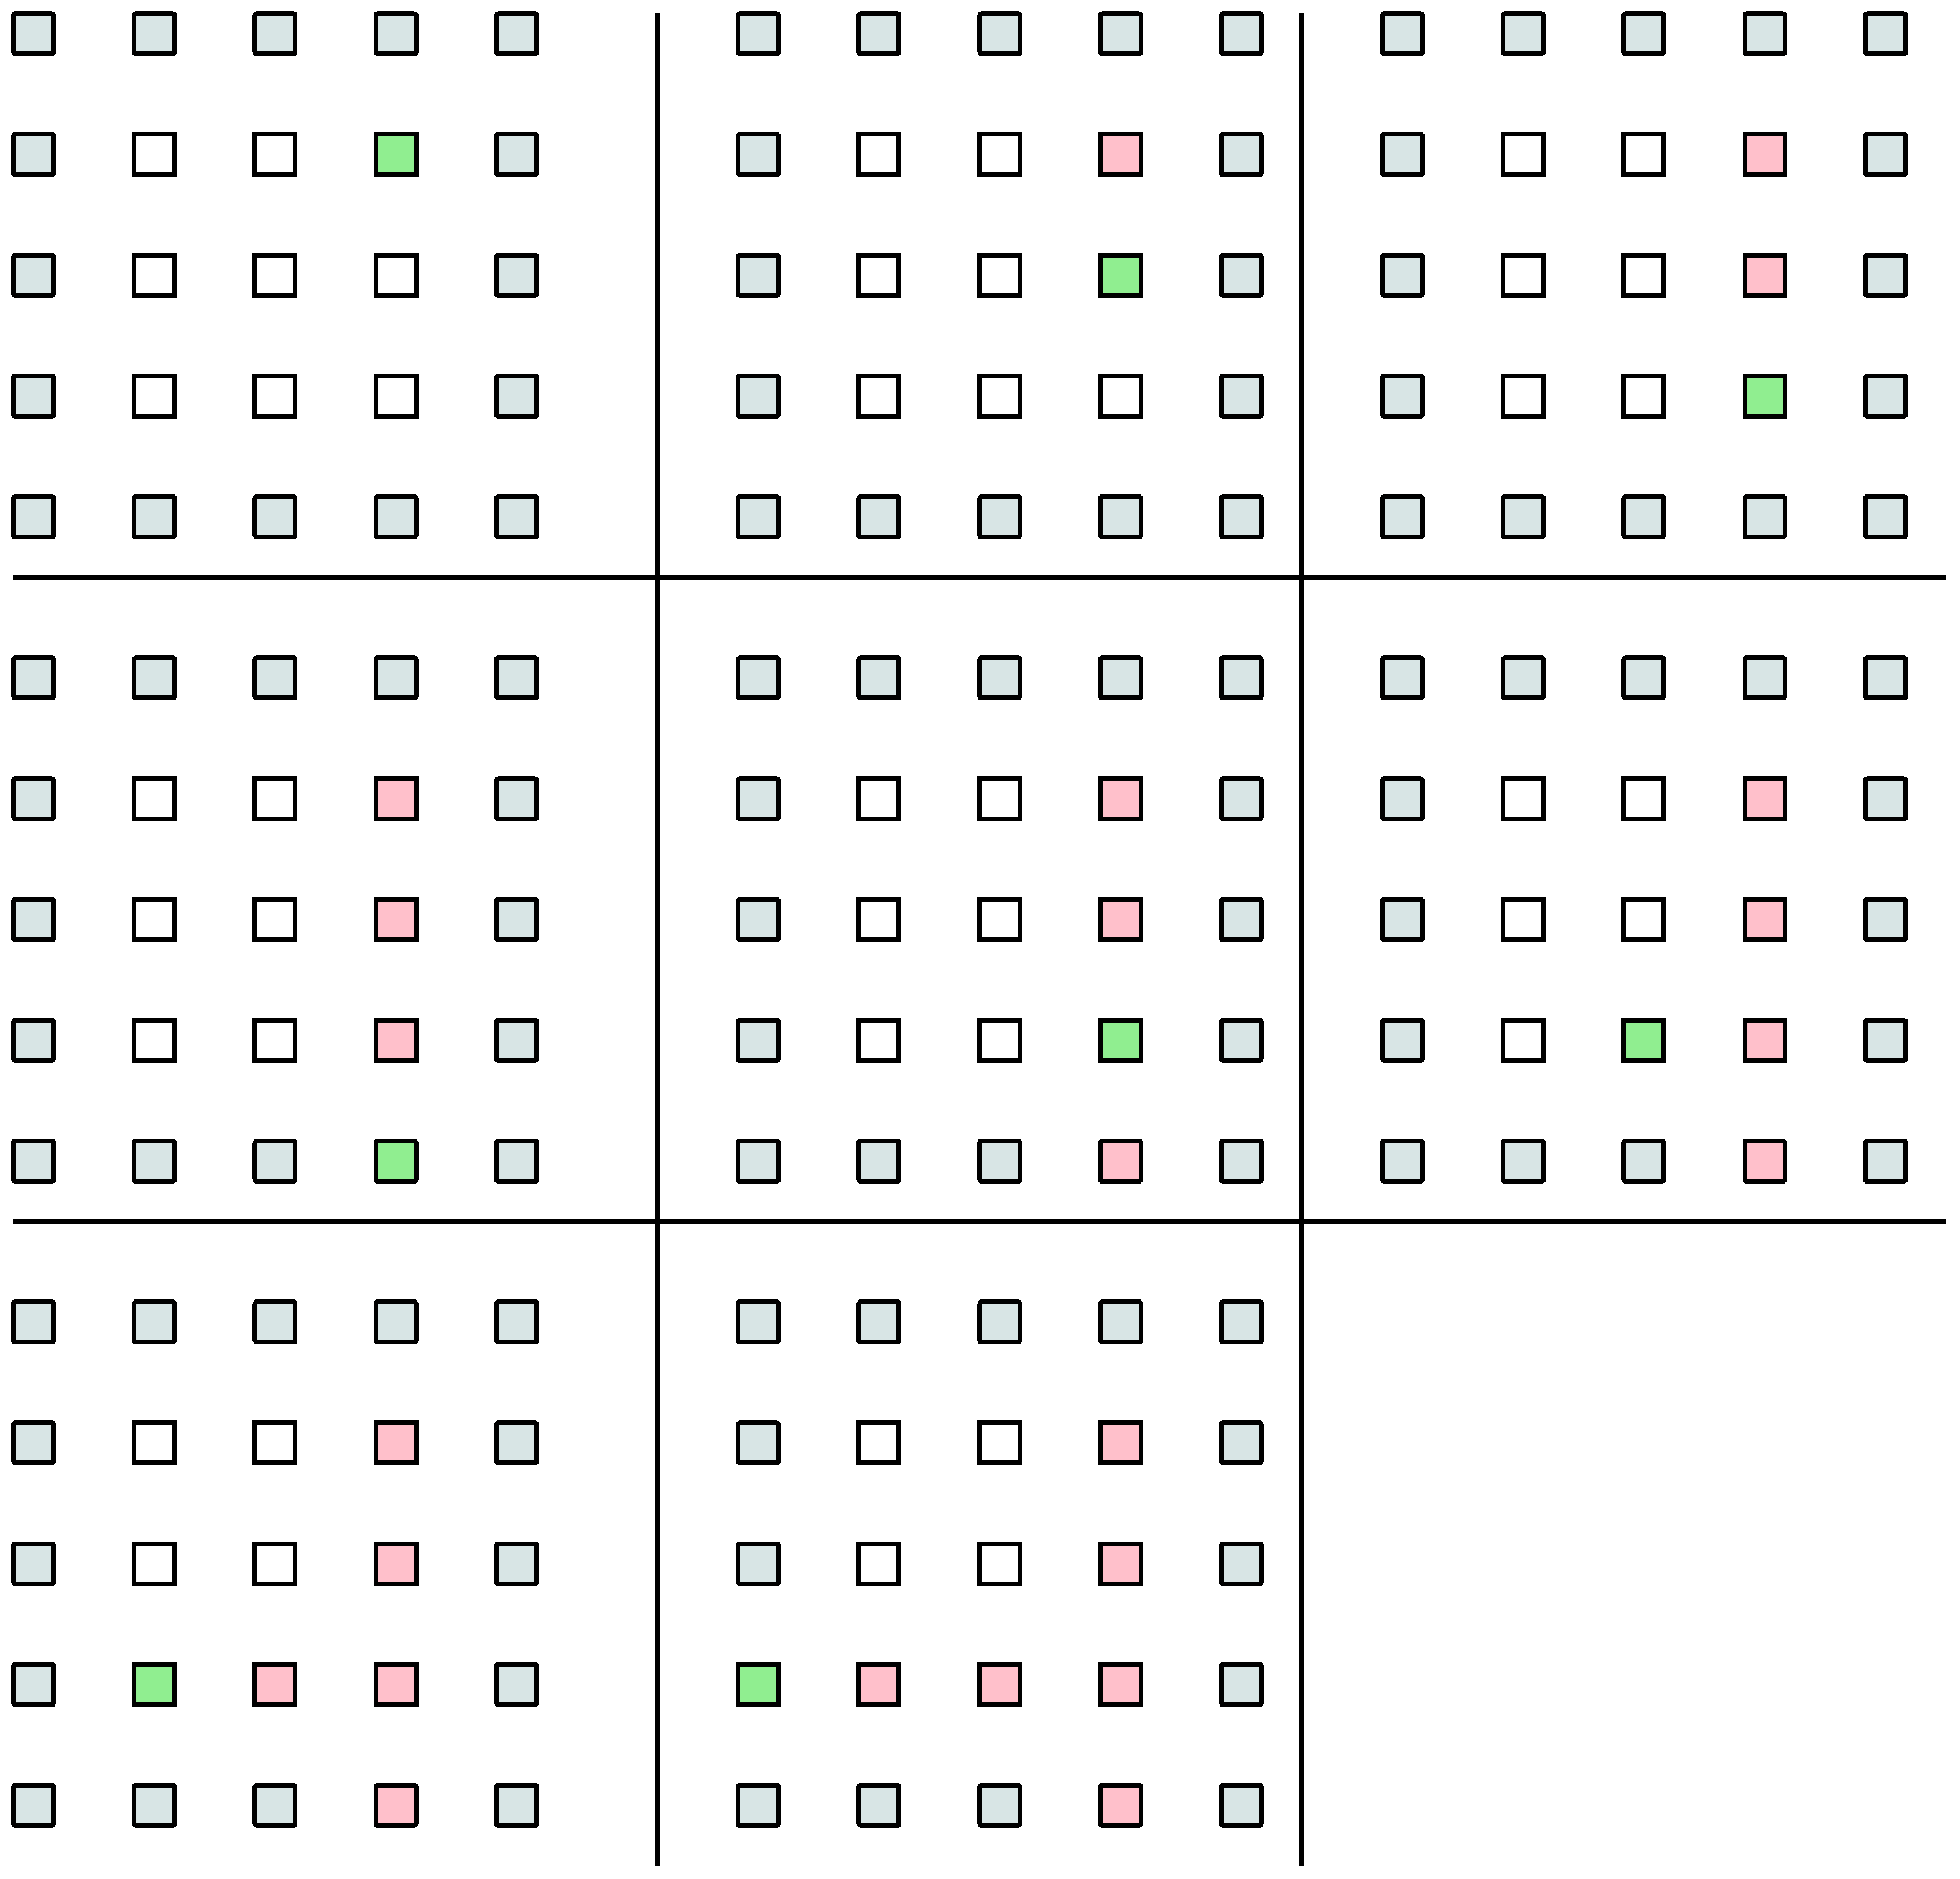
\includegraphics[width=0.5\textwidth]{find_corner}
\caption{How the agent finds the corner}
\end{figure}

After finding the bottom left corner the agent starts the actual algorithm. The
algorithm moves the agent in an S shape. Being in the bottom left corner the
agent will start the first swipe to the right in the first row.	Once the agent
hits the bottom right corner the agent will move one row up, and start the swipe
number 2, to the left.	The variable swipeNumber is used to control in which
direction the agent should go.	If the swipeNumber is an odd number the agent
moves to the right until it find the wall. If it's an even number it moves to
the left.	When the agent hits the top wall it starts going down to find the
bottom row.	Once in the bottom row the number of swipes is increased again and
the agent starts again the algorithm.	In the figure is easy to see how the agent
moves, each of the red lines will be a movement and the green lines are the
reaction of the agent after finding a wall.


\begin{figure}[h]\label{fig:simpleAlgorithm} \centering
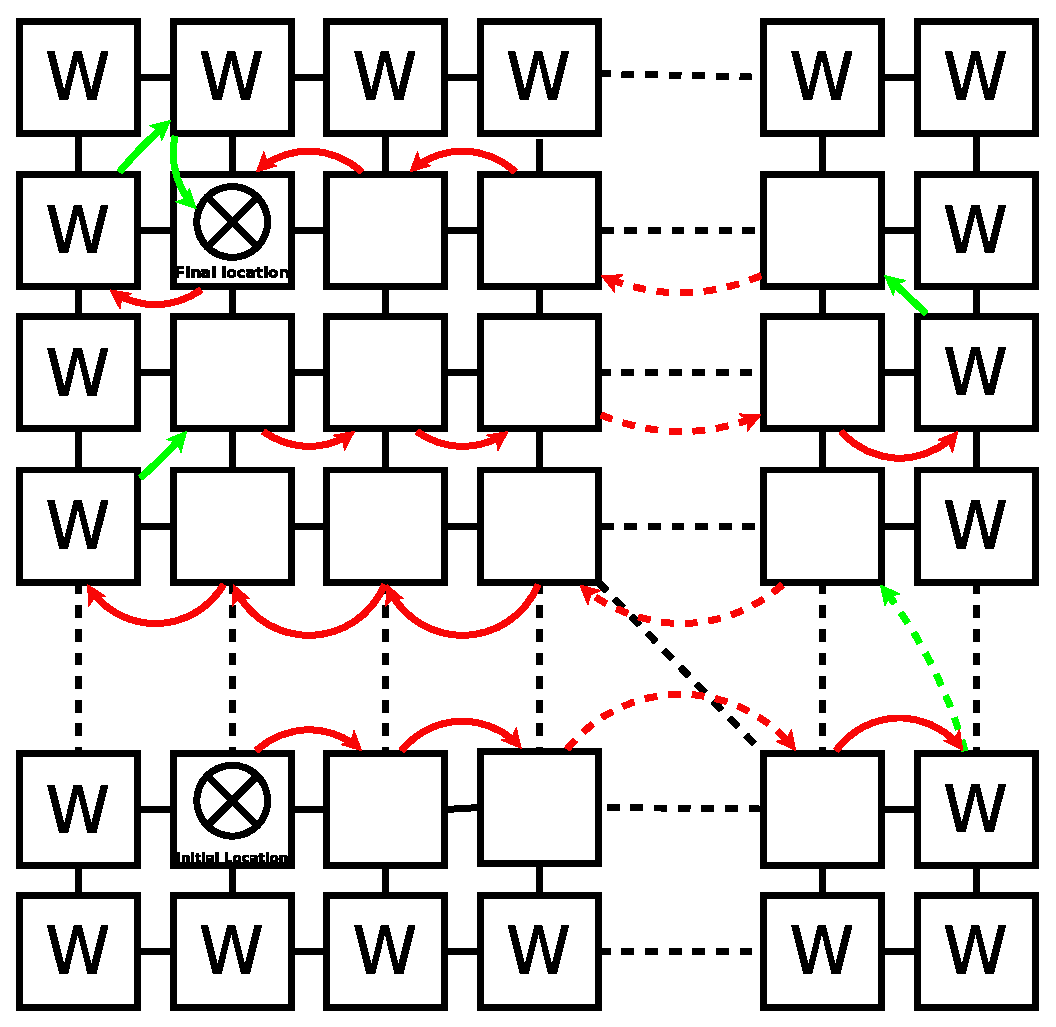
\includegraphics[width=0.5\textwidth]{SimpleAlgorithm}
\caption{How the agent moves}
\end{figure}


\subsubsection{Performance test - initial dirt}
For this performance test the environment receives its random dirt during
creation and, the agent will stop after finding all of the four corners

\begin{longtable}{p{0.05\textwidth} p{0.075\textwidth} p{0.075\textwidth} 
									p{0.13\textwidth}}
Steps & Moves & Cleans	& Performance \\\hline
1000 & 25 & 6 & 11927 \\
 & 25 & 6 & 10930	\\
 & 25 & 4 & 10966	\\
 & 25 & 7 & 11896 \\
 & 25 & 4 & 11951 \\\hline
AVG		& 25 &  5	 & 11534	\\\hline
\end{longtable}



	
\section{Task C}
According to the book, for each possible sequence, a rational agent should
select an action that is expected to maximize its performance measure. If it
deducts one point for each movement, the agent should require a memory because
it should remember in which cells has been, and it won't visit those cells
again. In this way there will be less moves. Because, if the agent does not know
in which cells has been before, it will visit them again, and the number of
movements will increase.

So, we think that the agent should require an internal state because it will
prevent the agent from visiting the same cells and it would reduce needless
movements and loss of points.





	
\section{Task D}
Yes of course. The agent should learn the environment from its experience. It
should learn how much time does it takes after e cell is cleanded to get dirty,
so it would know when should it go back to clean it again. In this way the
efficiency will increase.


	
\section{Task E}
\subsection{Two-cell environment}
\subsubsection{Environment description}
\t This is the basic environment, with only two cells. The two cells are manually
created and they only point one to each other. This means that the only neighbor
of the left cell is the right cell and viceversa.

The dirty state of each cell is randomly updated with a probability of the 20\% 
of getting dirty. One out of 5 times the cell gets dirty.

\subsubsection{Agent description}
\t The agent implementation for the two cell environment is easier than for
bigger or more complex environments. 

In this case the agent has less states. It can be placed in a clean cell working,
then it will move to the other cell. If it is in a dirty cell it will suck it. 
If it is off he will do nothing.

\subsubsection{Random dirt performance test}
This test case is the same as previous, but here the environment will receive
randomly generated dirt at the start of each step before the agent perceives the
location.  Then if it has covered all the cells, it will stop and wait for
a maximum of 3 steps or until its current location becomes dirty. Then it will
restart it self and go over the environment once more. This continues until the
number of steps has reached the maximum amount.  They stay very similar because
of the RNG-method chosen. Which is using the ctime library, seed the RNG with
time(0), and generate a random number which is limited with modulus 5.

Because of this modulus 5, it will generate dirt extremely often and thus
resulting in a low performance.  A clean cell will because of this have a 20\%
chance of becoming dirty after each step.

Each test is run three times to yield some comparison of its randomized dirt
generation.

\begin{longtable}{p{0.05\textwidth} p{0.075\textwidth} p{0.075\textwidth} 
									p{0.05\textwidth} p{0.075\textwidth} p{0.075\textwidth} 
									p{0.13\textwidth}}
Start	& A & B & Steps & Moves & Cleans & Performance \\\hline
A & Clean & Clean & 1000 
		 & 239 & 279 & 1480 \\
	&&&& 233 & 305 & 1404 \\
	&&&& 241 & 292 & 1423 \\
	&&&& 238 & 287 & 1378 \\
	&&&& 231 & 309 & 1426 \\\hline
  &&& AVG & 236.4 & 294.4 & 1422.2\\\hline

B & Clean & Clean & 1000 
		 & 236 & 279 & 1437 \\
	&&&& 236 & 317 & 1412 \\
	&&&& 236 & 306 & 1412 \\
	&&&& 240 & 290 & 1478 \\
	&&&& 244 & 308 & 1474 \\\hline
  &&& AVG & 238.4 & 300.0 & 1442.6 \\\hline
\end{longtable}

\subsection{Simple environment}
\subsubsection{Environment description}\label{sec:SimpleEnvDesc}
\t We created an environment of 5 rows consisting of 6 cells each. The outer layer of
cells are set to walls and there are no obstacles within. That makes a rectangular
inner shape of 3 rows and 4 columns. 

The dirt spread around the environment is randomly generated every time the main
program updates. The probability that a cell gets dirty is 20\%\. This means that the
cell will become dirty once every 5 times it gets updated.


\subsubsection{Agent description}
\t The agent in the simple environment it's the basic agent we programmed called
dummyAgent aka Bender. This agent uses the S algorithm to go trhough the hole
environment.

In the simple environment as explained in section \ref{sec:SimpleEnvDesc} The dirt
 state in the cell is updated. With this condition, the agent stops working once he
 found all the four corners. When the current location becomes dirty or he has being
 waiting for 3 cycles he will reboot and start cleaning again. By waiting this time 
 we make sure that the agent doesn't move over just cleaned cells.

\subsubsection{Performance test - updated dirt}
\t For the performance test we created an environment of 5 rows consisting of 6
cells each.  The outer layer of cells are set to walls and there is no obstacles
in the environment.  The dirt is randomly generated from the start and the agent
does not maintain a log of the environment, nor where it's been. It follows the
algorithm by finding the corner and then continuing by making passes side to
side and work its way up and down.  It will pause each time it has found all
four corners, the pause is a maximum of 3 steps or untill the location becomes
dirty.

The grid is a 5 by 6 matrix, outer layer is walls and the inner area is a 3 by 4
matrix where dirt is randomly generated.

In this case the chances of a clean cell becoming dirty again during a step is
20\%\.  This means the rate of clean cells becoming dirty again is extremely
likely and therefore resulting in such a low performance since the perfect
performance would be 12.000.

\begin{longtable}{ p{0.05\textwidth} p{0.075\textwidth} p{0.075\textwidth} 
									 p{0.13\textwidth} }
Steps & Moves & Cleans	& Performance \\\hline
1000	& 525 & 444 & 2214 \\
 		 	& 535 & 434 & 2102 \\
 			& 537 & 431 & 2197 \\
 			& 531 & 438 & 2163 \\
 			& 522 & 447 & 2328 \\\hline
AVG		& 530 & 438 &	2200 \\\hline
\end{longtable}


\subsection{Recursive agent - Theoretical}
\subsubsection{Environment description}

\subsubsection{Agent description}

\subsubsection{Performance test - updated dirt}




	\section{Reason for low performance}
		Our method for allocation dirt will allocate dirt to a cell wil 20\%\ chance
		of creating it in the current location.  This means that the envinorment
		will almost continously add dirt to the environment after the cell has been
		cleaned.

		This means that the agent basically can't clean the environment fast enough
		to have a good performance rate
\end{document}
